%Latex2e file
\documentclass[12pt,letterpaper]{article}
%\renewcommand{\arraystretch}{2}
%\input{\scrload.tex}
\setlength{\textwidth}{6.5in}
\setlength{\textheight}{8.6in}

\setlength{\oddsidemargin}{-.25in}
\setlength{\evensidemargin}{-.25in}
\setlength{\topmargin}{-.25in}
\pagestyle{empty}

\usepackage{amsmath}
\usepackage{amssymb}
\usepackage{graphicx}

\newcommand{\R}{\ensuremath{{\mathbb{R}}}}
\newcommand{\Z}{\ensuremath{{\mathbb{Z}}}}
\newcommand{\Q}{\ensuremath{{\mathbb{Q}}}}
\newcommand{\N}{\ensuremath{{\mathbb{N}}}}
\newcommand{\C}{\ensuremath{{\mathbb{C}}}}
\newcommand{\Proof}{\noindent {\bf Proof: }}
\newcommand{\QED}{\begin{flushright}QED\end{flushright}}
\newcommand{\Refl}{{\bf Reflexive: }}
\newcommand{\Symm}{{\bf Symmetric: }}
\newcommand{\Tran}{{\bf Transitive: }}
\newcommand{\ep}{\varepsilon}
\newcommand{\ri}{\right|}
\newcommand{\lef}{\left|}
\newcommand{\toR}{\to \R}
\newcommand{\fancy}[1]{#1_{\text{fancy}}}
\newcommand{\pro}[1]{\noindent {\bf #1}}
\newcommand{\prob}[1]{\newpage\noindent {\bf #1}}
\newcommand{\bacon}{\approx}

   
\begin{document}
\begin{flushright}
Nick Kerner

Homework 8

Chapter 6: 9

Dr Frey's Bonus but required fun question

Chapter 7: K2, K3, K5

\end{flushright}
\begin{center}
\large{Geometry}\\
\end{center}

\pro{Chapter 6: problem 9 }

Given $X\neq P $ on l, by proposition 6.6 we know there are two limiting parallel rays to $l'$ emanating from P (on opposite sides of $\overleftrightarrow{PQ}$.  Choose the one on the same side of $\overleftrightarrow{PQ}$ as X and drop a perpendicular from X to our limiting parallel ray and call the foot Y.   Know we know that $\overrightarrow{PY}$ is interior to $\angle QPX$ ($\overrightarrow{PY}\neq \overrightarrow{PX}$ as limiting parallel rays cannot have a common perpendicular to their respective line by Hilbert's Hyperbolic axiom of parallels, so XY is a segment not a point). \\

Case 1: $\overrightarrow{PY}$ is interior to $\angle XPX'$\\

Then by crossbar theorem we know that $\overrightarrow{PY}$ must intersect $XX'$. \\

Case 2: $\overrightarrow{PY} = \overrightarrow{PX'}$\\

Our limiting parallel cannot intersect $l'$.  Contradiction.\\

Case 3: $\overrightarrow{PY}$ is interior to $\angle QPX'$.\\

By crossbar theorem, $\overrightarrow{PY}$ intersects $QX'$, but our limiting parallel cannot intersect $l'$.  Contradiction.\\

Therefore we know that $\overrightarrow{PY}$ intersects $XX'$ (not at an endpoint as it would be the parallel with common perpendicular to $l'$ or it would intersect $l'$) call this point Z.  \\

Case 1: Y = Z.\\

$XY = XZ$, clearly. \\

Case 2: $Y\neq Z$.\\

Consider $\triangle XYZ$.  We know that $\angle XYZ$ is a right angle, so its measure is $90^\circ$, so since we are in hyperbolic a triangle's angle sum must be less than 180, so both other angles have measures less than $90^\circ$.  So we know by proposition 4.5 that since $\angle XYZ > \angle XZY$ then $XZ > XY$.\\

Hence $XZ \geq XY$.\\

To use Aristotle's axiom, we must show that $\angle XPY$ is acute. Now we know that $\angle QPY$ is acute (proposition 6.6) and we know that it is interior to $\angle QPX$ which is right, so by angle subtraction we know that $\angle XPY$ is acute. \\

By Aristotle's axiom, given any segment AB (A on l, B on $\overrightarrow{PY}$), there is some X with foot Y such that $XY > AB$.  So we know by segment addition that $XX' > XZ \geq XY > AB$. 

\QED 



\prob{Dr Frey's Bonus but required fun question }

%AMN is not similar to ABC
\Proof

Assume to the contrary that $\delta (AMN) = \delta (ABC)$. By proposition 6.1 we know that $\delta (ABC) = \delta(MCB) + \delta (MCA)$.  Additionally we know that $\delta (MCA) = \delta (MNC) + \delta (AMN)$, so we know that $\delta (ABC) = \delta(MCB) + \delta (MCA) = \delta(MCB) + (\delta (MNC) + \delta (AMN)) = \delta(MCB) + \delta (MNC) + \delta (ABC)$.  Therefore $\delta (MCB) + \delta (MNC) = 0$ so $\delta (MCB)= 0$ and $\delta (MNC) = 0$.  Contradiction.  Hence $\triangle AMN$ and $\triangle ABC$ cannot be similar. 

\QED


%MN \not \cong BL
\Proof

Assume to the contrary that $MN \cong BL$.  Choose D such that $M*N*D$ and $ND \cong MN$. So $\angle CND$ and $\angle MNA$ are vertical angles, $MN\cong ND$ and $AN \cong NC$ so by SAS we know that $\triangle ANM \cong \triangle CND$.\\

So we know that $BM \cong MA \cong DC$.\\


Additionally we know that 

\begin{eqnarray*}
MD &=& MN + ND \\
&\cong & MN + MN \\
&\cong & BL + BL \\
&\cong & BL + LC\\
&=& BC
\end{eqnarray*}

and $MC \cong MC$ so by SSS we know that $\triangle MBC \cong \triangle CDM$.\\


Finally we know that $\angle BMC^\circ + \angle CMD^\circ + \angle DMA^\circ = 180$ as they make a straight line.  So (substitutions are either renaming angles or derived from congruent triangles).\\

\begin{eqnarray*}
180 &=& \angle BMC^\circ + \angle CMD^\circ + \angle DMA^\circ\\
&=& \angle MCD^\circ + \angle CMD^\circ + \angle DMA^\circ\\
&=& (\angle MCN^\circ + \angle NCD^\circ) + \angle CMD^\circ + \angle DMA^\circ\\
&=& \angle MCN^\circ + \angle NAM^\circ + \angle CMD^\circ + \angle DMA^\circ\\
&=& \angle NAM^\circ + \angle MCN^\circ + \angle CMD^\circ + \angle DMA^\circ\\
&=& \angle NAM^\circ + \angle MCN^\circ + \angle MCB^\circ + \angle DMA^\circ\\
&=& \angle NAM^\circ + (\angle MCN^\circ + \angle MCB^\circ) + \angle DMA^\circ\\
&=& \angle NAM^\circ + \angle NCB^\circ + \angle DMA^\circ\\
&=& \angle CAB^\circ + \angle ACB^\circ + \angle DMA^\circ\\
&=& \angle CAB^\circ + \angle ACB^\circ + \angle MDC^\circ\\
&=& \angle CAB^\circ + \angle ACB^\circ + \angle CBM^\circ\\
&=& \angle CAB^\circ + \angle ACB^\circ + \angle CBA^\circ
\end{eqnarray*}

So $\delta (ABC) = 0$.  Contradiction.


\QED





\prob{Chapter 7: K2 }

a. 

\begin{center}
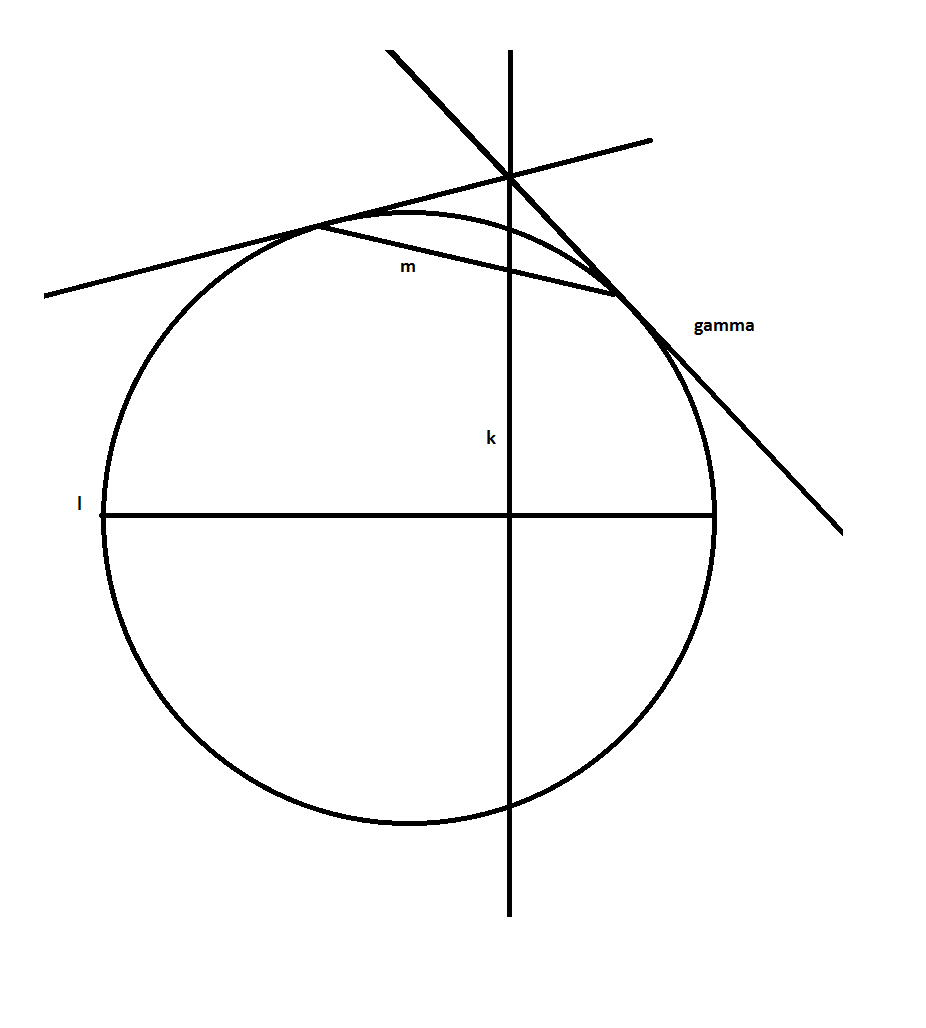
\includegraphics[width=2in]{klein2.png}
\end{center}


b. 

\begin{center}
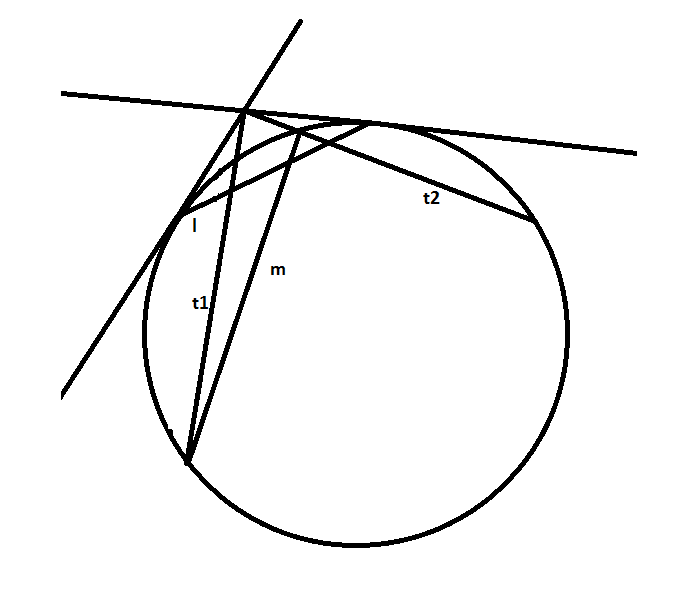
\includegraphics[width=2in]{klein2b.png}
\end{center}

Case 1: l is a diameter.  Then both lines perpendicular to l make a right angle with l.  So using m, l and 1 of these lines to construct a triangle, you can see that the angle between the transversal and m must therefore be acute.

Case 2: m is a diameter (l is not)





\newpage

c. 


\prob{Chapter 7: K3 }

\prob{Chapter 7: K5 }



\end{document}